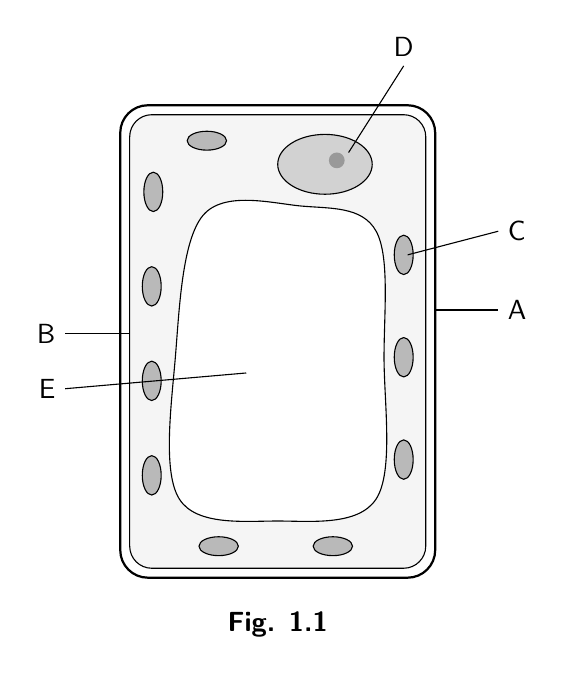
\begin{tikzpicture}[scale=1.0, font=\sffamily, line join=round]
  \draw[thick, rounded corners=10pt, fill=white] (0,0) rectangle (4,6);           % cell wall
  \draw[thin, rounded corners=8pt, fill=gray!8] (0.12,0.12) rectangle (3.88,5.88); % cell membrane + cytoplasm
  \draw[fill=white] plot[smooth cycle, tension=0.6] coordinates {(0.75,1.0) (2.0,0.72) (3.25,1.0) (3.35,2.8) (3.25,4.4) (2.3,4.72) (1.05,4.6) (0.7,2.8)}; % vacuole
  \draw[fill=gray!35] (2.6,5.25) ellipse (0.6 and 0.38);  % nucleus
  \fill[gray!80] (2.75,5.3) circle (0.1);
  \foreach \x/\y/\r in {0.4/1.3/90, 0.4/2.5/90, 0.4/3.7/90, 0.42/4.9/90, 3.6/1.5/90, 3.6/2.8/90, 3.6/4.1/90, 1.25/0.4/0, 2.7/0.4/0, 1.1/5.55/0}
    \draw[thin, fill=gray!55, rotate around={\r:(\x,\y)}] (\x,\y) ellipse (0.25 and 0.12);
  \draw (4,3.4)--(4.8,3.4) node[right] {A};
  \draw (0.12,3.1)--(-0.7,3.1) node[left] {B};
  \draw (3.65,4.1)--(4.8,4.4) node[right] {C};
  \draw (2.9,5.4)--(3.6,6.5) node[above] {D};
  \draw (1.6,2.6)--(-0.7,2.4) node[left] {E};
  \node[font=\sffamily\bfseries] at (2,-0.6) {Fig. 1.1};
\end{tikzpicture}
